\documentclass[a4paper,12pt]{article}
\usepackage[utf8]{inputenc}
\usepackage{blindtext}
\usepackage{enumitem}
\usepackage{index}
\usepackage{graphicx}
\usepackage[portuguese]{babel}
\usepackage{indentfirst}
\usepackage{multicol}

\makeindex

\title{Projeto-Relatório}
\begin{document}
\maketitle
\begin{center}
    
\includegraphics[width=6cm]{imagens/uminho.png}
    \vspace*{0.5cm}
\end{center}

\begin{center}
\author{grupo 16: \\ Cláudia Silva, a93177 \\ João Mendes, a93256 \\ André Vaz, a93221 \\ Tomás Ogando, a93174}
\end{center}

\pagenumbering{arabic}

\newpage

\tableofcontents

\setcounter{page}{2}


\newpage


\section{Introdução}
	Na primeira fase deste trabalho pretendeu-se desenvolver um sistema  de  representação  de  conhecimento  e raciocínio com capacidade para caracterizar um universo de discurso na área da logística de distribuição de encomendas. Para tal tivemos de desenvolver um sistema de encomendas para uma empresa denominada por \emph{Green Distribution} que tem como objetivo privilegiar a ecologia acima de tudo. Cada estafeta desta empresa foi associado a diversas encomendas podendo utilizar três possíveis transportes. Tendo isto em consideração, elaboramos diversas funções em \emph{Prolog} que, utilizando a base de dados criada por nós, dão-nos acesso a várias informações.\par
	Com isto, decidimos optar para uma melhor pratica dividir o projeto criando dois ficheiros \emph{Prolog}: \emph{basedados.pl}, onde estão presentes os predicados e conhecimento que sustentam o trabalho e \emph{queries.pl} onde estão implementadas todas as funcionalidades propriamente ditas.\par

\newpage

\section{Base de Conhecimento}
	Nesta primeira fase começamos por definir a base de dados. Consideramos 6 estafetas (Cátia, Carlos, Sheila, Ilídio, Filipe e Roger) e 6 clientes (Ogando, Paulo, Marlene, Susana, Jéssica e Sandro) cada um tendo uma rua associada e,  consequentemente, cada uma das ruas uma freguesia associada. Relacionamos também um índice de poluição a cada veículo, desta forma pudemos mais facilmente descobrir quem utiliza mais vezes o meio de transporte mais ecológico, sendo util para \emph{query} 1. De facto, consideramos que o nível de poluição da bicicleta era 0 (uma vez que ela não causa poluição), o nível de poluição do carro era 2 e da mota 1. Desta maneira, assumimos que uma viagem carro polui tanto quanto duas de mota.\par
	Em relação ao conteúdo das encomendas, decidimos adotar 4 tipos diferentes. Cada um dos tipo tem um peso e um volume associados. Há a possibilidade de transportar livros, roupa, um computador e uma bicicleta. Isto permitiu-nos realizar com mais facilidade a última \emph{query} proposta em que tinhamos que calcular o peso total transportado num dia.\par
	Além disso, criamos o caminho, que nos indica várias informações. Na verdade, através do facto \emph{caminho} sabemos quem foi o cliente, o estafeta que vai realizar a entrega, o veículo que vai ser utilizado, a data e hora que foi encomendado, o que leva a encomenda, o preço de transporte, o espaço de tempo em que o cliente a quer receber e o número de série da mesma. Dessa forma, ao associar o número de série a cada encomenda garantimos que não há uma repetição da mesma entrega (assim se um cliente realizar duas encomendas seguidas garantimos que são distintas). Foi também criada a confirmação dos factos para conseguirmos comparar as encomendas ainda por completar. Com estas confirmações temos acesso aos dados de cada encomenda, nomeadamente, a data de entrega da mesma, o \emph{ranking} e o tempo que demorou a ser entregue. Posteriormente, ajudam-nos a confirmar resultados sobre que estafeta fez determinada entrega.\par
	Para as \emph{queries} 7, 8 e 9 em relação aos intervalos de tempo decidimos considerar dias para obter o resultado, comparando a data de saída com a data de chegada.\par
    Fomos encorajados a incluir novas funcionalidades neste projeto e decidimos aceitar o desafio desenvolvendo duas novas funcionalidades. A primeira adição ao projeto trata-se de uma forma de descobrir que entregas foram feitas numa determinada hora. Utilizando funções e métodos de resolução aplicados previamente, conseguimos implementar esta query. Além disso, também criamos uma forma de descobrir quais as encomendas entregues a horas e das encomendas em falta.\par
    
\section{Queries}
    
    \subsection{Query 1}
        Na \emph{query} 1 tinhamos como objetivo obter o estafeta que utilizou mais vezes um veiculo mais ecologico, sendo este a bicicleta.\par
        Deste jeito, começamos por definir o predicado \emph{query1\_aux} que recebe um estafeta e devolve o número de vezes que o mesmo utilizou como meio de transporte uma bicicleta. Assim, tendo a lista de todos os estafetas podemos calcular o número de vezes que cada um deles utilizou a bicicleta, sendo isto feito através da \emph{query1\_tuple}. Tendo os valores para cada estafeta falta apenas orderar a lista de forma a que o estafeta com maior valor fique em primeiro, sendo isto realizado na função \emph{compare\_by\_second}, podendo então concluir que o estafeta mais ecológico é o que estiver em primeiro na lista.
    
        \begin{center}
            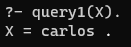
\includegraphics[scale=1]{imagens/query1.png}
        \end{center}
        
    \subsection{Query 2}
        Para identificar que estafetas entregaram determinada(s) encomenda(s) a um determinado cliente optamos por criar duas funções.\par
        Primeiramente, o predicado \emph{query2\_aux} que dado um cliente e uma encomenda vai descobrir o estafeta que a realizou e verificar o número de série. De seguida, confirma se essa encomenda foi entregue .Posteriormente, averigua se se trata de um estafeta. Na função  \emph{query2}, com o auxilio da função \emph{findall} conseguimos aplicar a \emph{query2\_aux} a todos os caminhos.\par
        
        \begin{center}
            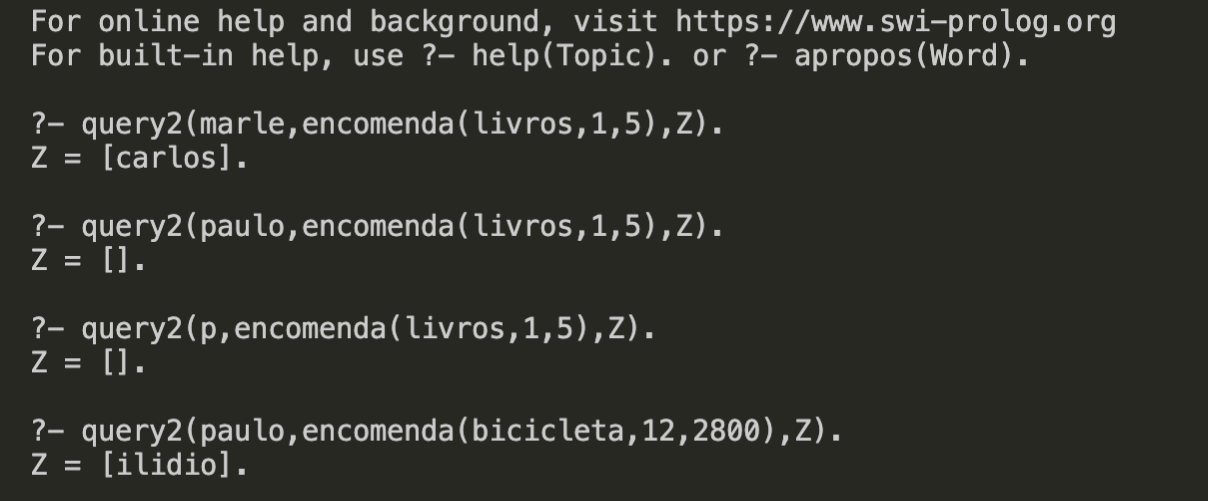
\includegraphics[scale=0.6]{imagens/query2.png}
        \end{center}
    
    \subsection{Query 3}
        Para esta query \emph{query} foi necessário identificar os clientes que foram servidos por um determinado estafeta dado pelo utilizador. Inicialmente, verifica se existe alguma entrega feita pelo estafeta a um determinado cliente através da \emph{query3\_aux}, que nos vai permitir depois na \emph{query3} desenvolver uma lista com os clientes.\par
    
        \begin{center}
            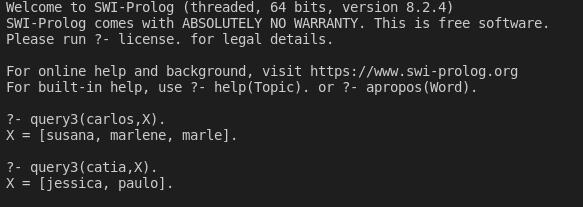
\includegraphics[scale=0.6]{imagens/query3.png}
        \end{center}
        
    \subsection{Query 4}
        A estratégia usada para saber o valor faturado pela \emph{Green Distribution} num determinado dia consiste no desenvolvimento de uma auxiliar, \emph{soma}, que tem como objetivo final somar todos os elementos da lista. Assumimos que o cliente paga mal faça a encomenda, assim sendo trabalhamos com o facto \emph{caminho} para verificar se existe o dia e o preço inseridos pelo utilizador.\par
        Por fim, desenvolvemos a \emph{query4} com o objetivo de  identificar o valor calculado, através da auxiliar soma e também pelo \emph{findall} que nos permitiu juntar tudo numa lista para que a soma fosse possivel.\par
    
        \begin{center}
            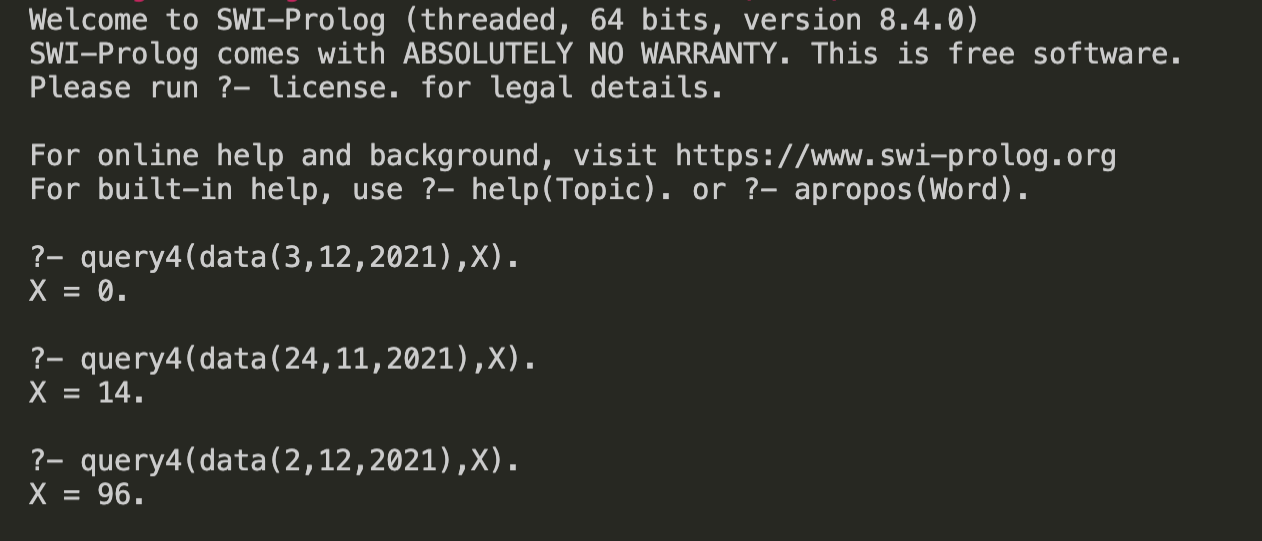
\includegraphics[scale=0.6]{imagens/query4.png}
        \end{center}
    
    \subsection{Query 5}
        Para a resolução desta \emph{query} decidimos desenvolver várias auxiliares que ajudassem no processo para identificar as zonas com maior volume de entregas por parte da empresa \emph{Green Distribution}. Assim sendo, numa primeira fase, desenvolvemos \emph{query5\_aux2} que agrupa numa lista todas as ruas existentes, através do \emph{findall}. De seguida desenvolvemos uma auxiliar que tem o intuito de procurar uma dada rua numa lista com as ruas todas e agrupar o respetivo nome da rua consoante as vezes que aparece na lista, \emph{procura}. A partir desta, conseguimos desenvolver a \emph{query\_comp} que organiza as ruas pela cabeça da lista. Através do desenvolvimento da \emph{compare\_by\_second2} que compara de forma descrescente e da \emph{query\_comp}, como já foi referida, elaboramos a \emph{query5\_aux1} que organiza a lista de ruas de forma descrescente consoante o número de vezes que aparecem.\par
        Por fim, a \emph{query5} devolve a cabeça da lista que corresponde ao local com maior volume de entregas.
        
        \begin{center}
            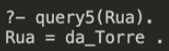
\includegraphics[scale=0.9]{imagens/query5.png}
        \end{center}
        
    \subsection{Query 6}
        A resolução desta \emph{query} consiste em calcular a classificação média de satisfação de clientes num determinado estafeta. Assim sendo, decidimos fazer uma lista com o número de viagens que determinado estafeta fez, por isso usamos o \emph{length}. Para calcular a soma de todas as avaliações feita aos estafetas, agrupamos a avaliação numa lista e somamos. Por último, tendo o número de viagens realizadas por estafeta e a soma de todas as avaliações dessas viagens dadas pelos clientes, calculamos a média como é pedido.\par
    
        \begin{center}
            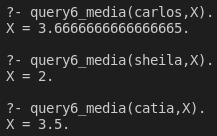
\includegraphics[scale=0.8]{imagens/query6.png}
        \end{center} 
    
    \newpage
    \subsection{Query 7}
        Para identificar o número total de entregas realizadas pelos diferentes meios de transporte, num determinado intervalo de tempo optamos por criar uma função auxiliar que converte uma data para dias, a função \emph{convertDatatodays}. Posteriormente, é usada na função \emph{comp} que compara uma data e verifica se essa se encontra no intervalo indicado. Posto isto, a função \emph{aux} e \emph{query} 7 percorrem o facto \emph{confirmacao} "procurando" pelo veiculo indicado e verificando se a data se encontra entre o intervalo indicado, caso se encontre é acrescentada a uma lista que subconsequentemente é somado o tamanho. Para esta \emph{query} é necessário que seja inserida primeiro a data mais antiga e só depois a data mais recente.\par
    
        \begin{center}
            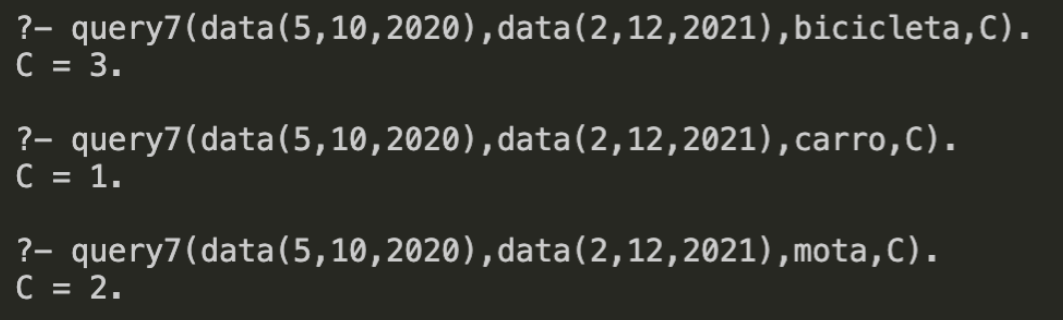
\includegraphics[scale=0.5]{imagens/query7.png}
        \end{center}

    \subsection{Query 8}
        Nesta \emph{query}, percorrendo o facto \emph{confirmacao} e comparando a data de cada um usando a função auxiliar \emph{comp}, usada na \emph{query} 7 conseguimos identificar o número total de entregas pelos estafetas, num determinado intervalo de tempo. Para esta \emph{query} é necessário que seja inserida primeiro a data mais antiga e só depois a data mais recente.\par
        
        \begin{center}
            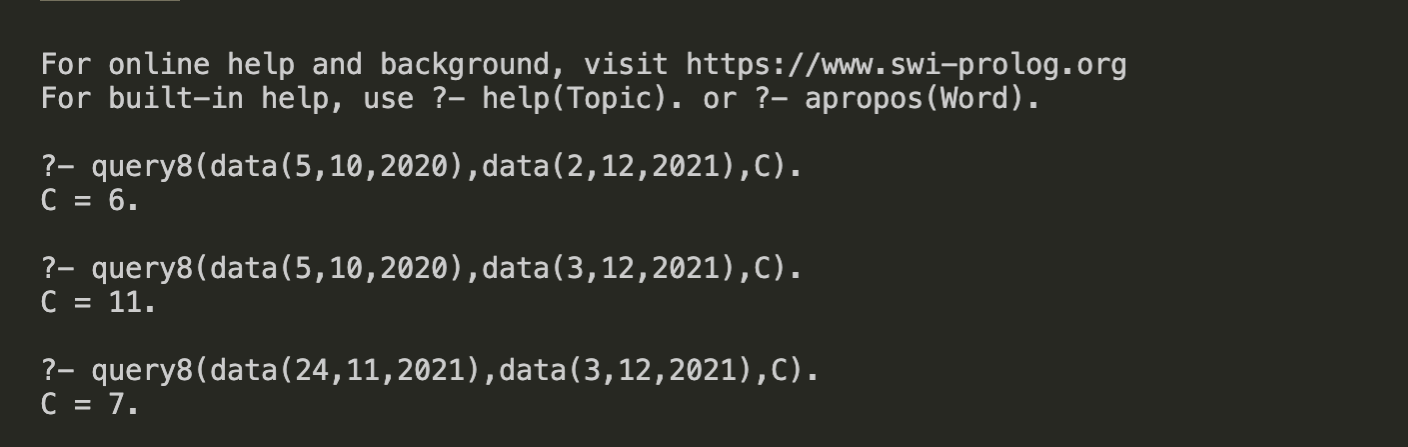
\includegraphics[scale=0.6]{imagens/query8.png}
        \end{center}

    \subsection{Query 9}
        A query 9 tem como objetivos calcular o número de encomendas entregues e não entregues pela \emph{Green Distribution}, num determinado período de tempo. Assim sendo, utilizamos a \emph{query} 8 como auxiliar uma vez que esta já identifica o número total de entregas pelos estafetas num determinado intervalo de tempo. Posteriormente, apenas contamos quantos factos \emph{caminho} existem e subtraimos as que foram entregues naquele intervalo de tempo ao total.\par
        
        \begin{center}
            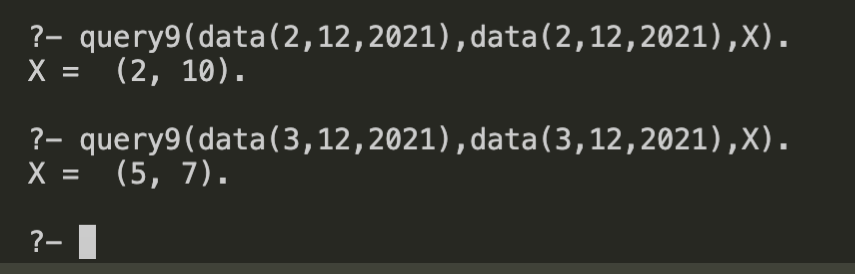
\includegraphics[scale=0.6]{imagens/query9.png}
        \end{center}
    
    \subsection{Query 10}
        Para o calculo do peso total transportado por um determinado estafeta num certo dia decidimos desenvolver duas funções.\par
        Primeiramente, criamos uma função auxiliar, \emph{query\_10} que tem como objetivo verificar se existe alguma encomenda que foi realizada consoante o estafeta ,dia e peso, através do facto \emph{caminho} e do facto \emph{confirmacao}.\par
        De seguida, baseamo-nos no mesmo processo de desenvolvimento feito para a \emph{query4}, que consiste em armazenar o peso numa lista através do \emph{findall} e, consequentemente, somar todos os elementos da lista para devolver o peso total num determinado dia.\par
        
        \begin{center}
            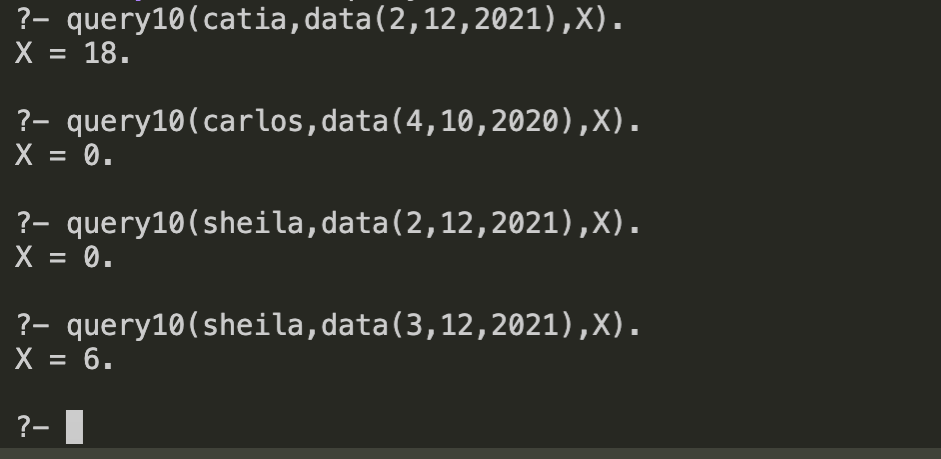
\includegraphics[scale=0.8]{imagens/query10.png}
        \end{center}
    
    \subsection{Query Adicionais}
        Nesta secção iremos abordar algumas \emph{queries} que decidimos elaborar.\par
    
        \subsubsection{Query Teste}
        A query teste verifica quantas encomendas foram, de facto, entregues.Ou seja,indica quantos caminhos tem a confirmação (usando o número de série). 
        \begin{center}
                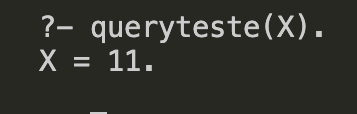
\includegraphics[scale=0.8]{imagens/queryteste.png}
            \end{center}
    
        \subsubsection{Query 11} 
            Elaboramos um facto que determinasse o número de entregas que ocorreram numa dada hora escolhida pelo utilizador. Para isso , através do \emph{findall} desenvolvemos uma lista com todas as encomendas que ocorreram numa dada hora e por intermédio do \emph{length} determinamos o tamanho da lista que corresponde ao número de entregas realizadas.\par
        
            \begin{center}
                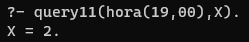
\includegraphics[scale=1]{imagens/query11.png}
            \end{center}
    
    
        \subsubsection{Query 12}
            Com o objetivo de obter uma lista com as diferentes entregas realizadas atempadamente, decidimos converter o tempo do facto \emph{caminho} e o tempo do facto \emph{confirmação} para horas, da seguinte maneira:\par
        
            \begin{center}
                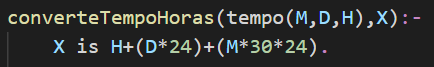
\includegraphics[scale=0.8]{imagens/query12/tempoHoras.png}
            \end{center}
        
            Com os tempos convertidos, podemos determinar se o tempo de confirmação é menor ou igual ao tempo do caminho, se tal o for então a entrega foi realizada atempadamente.\par
            Desta forma conseguimos concluir que as entregas que cumprem tal requisito são as seguintes:\par
    
            \begin{center}
                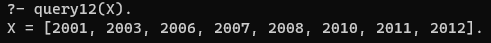
\includegraphics[scale=0.75]{imagens/query12/query12Res.png}
            \end{center}
        
        \subsubsection{Query 13}
            O invariante criado apenas deixa inserir um caminho se o número de série ainda não existir.
            
           
        \subsubsection{Query 14}
            Esta \emph{query} teve origem a partir da \emph{query1}, onde tem como resultado o estafeta que foi mais ecológico ao fim das entregas todas.\par
            
            \begin{center}
                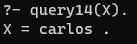
\includegraphics[scale=1]{imagens/query14.png}
            \end{center}
        
    \newpage
    \section{Conclusão}
	    Em arremate, este projeto permitiu-nos adquirir competências fulcrais no desenvolvimento de sistemas com capacidades de caracterizar um universo na área da logística de distribuição de encomendas. A utilização de uma linguagem como o \emph{Prolog} trouxe enúmeras vantagens na realização do projeto pois trata se de uma linguagem orientada à funcionalidade puramente lógica. Ademais, foi imprescindível o uso da nossa própria base de dados pois, permitiu uma maior liberdade de como abordar os problemas propostos. É opinião do grupo que esta fase foi concluída com sucesso.\par
    
    
    \newpage
    
\end{document}
    